
\chapter{Diskussion kring domänspecifika språk och fysik}

\begin{binge}

TODO: Nu när detta är mer resultat-aktigt måste det stilas om.

Hur en kombination av domänspecifika språk och fysik ser ut är för oss inte uppenbart. Går det att kombinera de två, och för vilka områden fungerar det bra för? Är det lärorikt att presentera fysik ur ett domänspecifikt-språk-perspektiv? Vi diskuterar här dessa frågor utifrån våra egna erfarenheter från projektet. 

\section{Om läromaterialets fokus på matematik och Haskell snarare än fysik}

En stor del av läromaterialets fokus ligger på matematik och Haskell snarare än fysik. Detta trots att läromaterialet är tänkt att handla om fysik. Varför är det så?

En orsak till att ett stort fokus ligger på matematik är att fysik egentligen bara är räkneexempel i matematik. Ta cirkulär centralrörelse som exempel. Att beskriva en sådan rörelse hos en kropp görs med hjälp av vektorer och matematisk analys. Fysik finns bara som en bakomliggande teori som dikterar vilka samband som gäller. Själva räknandet görs sedan med matematik.

Detta är dock inte hela sanningen. Inom fysik ingår en stor del problemlösning, till exempel att sätta upp och hitta krafter i mekanikproblem, utan att någon matematik behöver blandas in. Denna typ av fysik är dock svår att göra domänspecifika språk av, något som diskuteras djupare i avsnitt~\ref{sec:lampligt}.

Läromaterialet innehåller även en hel del förklaringar av Haskell-teknisk karaktär. Orsaken till detta är tvåfaldigt. För det första används avancerade koncept inom Haskell som läsaren inte förväntas kunna sedan innan. Ett exempel är typnivå-programmering. För att göra kopplingen mellan Haskell och fysik så tydlig som möjlig behövdes fysikaliska dimensioner kunna likställas med, och hanteras på samma sätt, som Haskell-typer.

För det andra är läromaterialets syfte inte enbart att lära ut fysik i sig, utan även visa hur fysik kan modelleras i domänspecifika språk och dra paralleller mellan fysik och domänspecifika språk. Av detta skäl blir det naturligt att det ''även'' ägnas en hel del förklaringar åt programkoden. Syftet är att väcka intresse för fysik, inte att lära ut fysik. Ett sätt att göra det är att visa dessa paralleller.

Är det rätt eller fel att ha en relativt liten tyngd på fysiken som projekets läromaterial har? På den frågan har vi mer än ett svar. Man kan svara ja, med hänvisning till de ovanstående skälen att det direkta syftet inte är att lära ut fysik utan att väcka intresse. Man kan svara nej, och hävda att de domänspecifika språken kan utformas på ett annat sätt som mer direkt knyter an till fysikaliska koncept, till exempel ett syntaxträd för sammansättningen av ett lutande plans komponenter. Vi tyckte dock det var svårt att göra på det sättet, se avsnitt~\ref{sec:lampligt}. Detta är dock en vidareutvecklingspotential, att undersöka huruvida det går att göra det på ett bra sätt.

Man kan också svara nej på frågan av ett annat skäl, nämligen att fysiken i sig bör vara det främsta fokuset. Detta skulle dock innebära en helt annan form på läromaterialet. Vi menar att det skulle vara svårt att väva in domänspecifika språk på ett meningsfullt sätt om de samtidigt skulle vara i skymundan. Ett läromaterial med större fokus på fysik bör i så fall enbart handla om fysik. En utförligare diskussion om detta finns i avsnitt~\ref{sec:bara_fysik}.

\section{Vad för slags områden är DSLs lämpligt att göra för?}
\label{sec:lampligt}

TODO: Hänvisa mer till resultat. Att av dessa skäl är inga DSLs för fysik.

Under projektets gång gjordes flera experiment för att se hur man kunde göra ett domänspecifikt språk för ett område. Det visade sig att visa områden var lämpligare än andra. Till exempel var analys och vektorer områden som vi ansåg väl lämpade, medan andra som till exempel lutande plan och termodynamik var mindre lämpade.

Vad har de lämpliga områdena gemensamt? De gemensamma dragen är att de är
matematiska, har en fix struktur och består av ``data och operationer''.
Tabell~\ref{tab:data_och_ops} visar några exempel på områden med sina data och
operationer.

\begin{table}[tph]
\centering
\caption{Exempel på data och operationer i några domänspecifika språk.}
\label{tab:data_och_ops}
\begin{tabular}{@{}l|l@{}}
\toprule
DSL / data & Exempel på operationer \\ \midrule
Dimensioner & Multiplikation, division \\
Vektorer & Addition, skalärprodukt \\
Analys, funktioner & Derivera, multiplicera \\ \bottomrule
\end{tabular}
\end{table}

Varför gör dessa drag att de är lämpliga att göra domänspecifika språk för?
TODO: Matematiska: man modellerar syntaxen

Den fixa strukturen kombinerat med data och operationer gör det enkelt att
modellera dessa områden med datatyper i Haskell. Datatyper har nämligen också en
fix form. Dessutom blir relationen mellan data och operationer i Fysik och
datatyper och funktioner i Haskell väldigt tydlig. En operation/funktion
resulterar sedan i data av samma slag som innan \todo{Som innan?}.

Denna strukturella likhet gör modellerandet och manipulerandet av data enkel att
genomföra rent tekniskt. Men den innebär också en pedagogisk vinst. Genom att ha
strukturerat upp fysik tydligt i Haskell blir det förhoppningsvis enklare för
läsaren att förstå hur datan hänger ihop rent fysikaliskt. Och även hur
relationerna mellan olika datatyper och funktionerna som dyker upp i
läromaterialet direkt kan översättas till relationer inom fysik.

I kontrast till dessa lämpliga områden står mindre lämpliga områden (eller
åtminstone områden som vi inte lyckades göra något bra av). Som nämndes tidigare
är termodynamik och lutande plan exempel på mindre lämpliga områden. Vad har
dessa områden för gemensamma drag?

Ett gemensamt drag som gör dem svåra att göra domänspecifika språk av är att de
består av en samling teoretiska samband. För det lutande planet är det till
exempel $a = g \cdot \sin(v)$, som illusteras i figur~\ref{fig:lutande_plan}.

\begin{figure}[tph]
  \frame{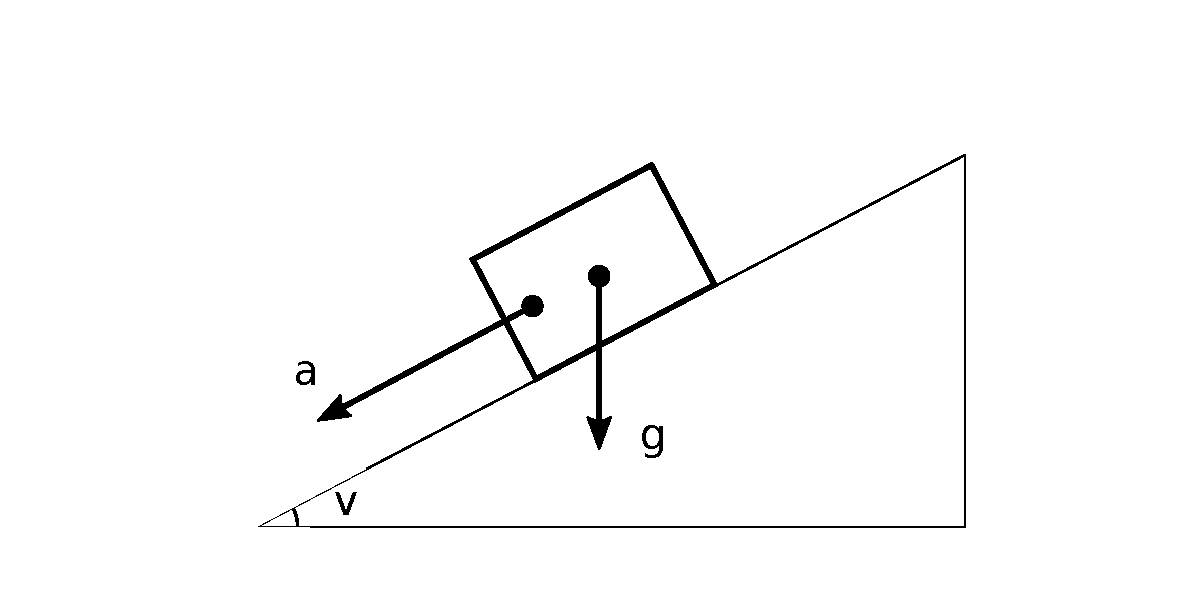
\includegraphics[width=\linewidth]{figure/Lutande_plan.pdf}}
  \caption{Den variant av lutande plan som referas till i exemplet i texten. $a$
  är en lådas acceleration längs med planet, $g$ är tyngdacceleration och $v$ är
  vinkeln. Friktionen antas vara försumbar.}~\label{fig:lutande_plan}
\end{figure}

Teoretiska samband av det slaget relaterar olika egenskaper i systemet.
Visserligen kan man modellera samband och ekvationer som ett domänspecifikt
språk, men vi menar att nyttan inte blir stor med det. Det man kan göra är att
programmera en ekvationslösare. Men den hade behövt vara både mekanisk och
komplex. Den skulle alltså skilja sig drastiskt från hur man löser problem för
hand och skulle vara svår att förstå. Alldeles för mycket fokus skulle hamna på
algoritmer istället för fysik.

När det kommer till lutande plan och liknande områden är nyckeln att visserligen
känna till vilka samband som gäller, men det framförallt att veta när man ska
använda dem och hur man tillämpar dem på olika typer av uppgifter. Vi behandlar
därför områden som lutande plan genom att lösa exempeluppgifter modellerade i de
tidigare domänspecika språk. De tidigare språken tillhandahåller de matematiska
verktyg som behövs för att koda upp lösningar av problem.


TODO: Kanske avsluta med att poängtera skillnaderna mellan lämpliga och mindre lämpliga.

Och vad är skillnaden mellan dessa två kategorier av områden?

Den viktiga skillnaden är att t.ex. analys har tydlig data och operationer 
medan problemlösning som lutande plan består av ett antal samband som används
beroende på behov. Dessa samband består då av koncept som redan är modellerade i
andra avsnitt och själva skrivandet av den koden bidrar inte med någon ny
kunskap som inte redan täcks av vanlig kurslitteratur inom fysik.

\section{Gör DSLs så att fysik blir mer lättförståeligt eller
intressant?}~\label{sec:bara_fysik}

TODO: Åke-möte2 gav viktiga insikter här som vi kan hänvisa till, utan att samtidigt få det att verka som Åke otvetydigt sagt att detta är bra utan att han verkar tycka att det kan vara något, efter en kort titt på det. För att "låta hans rygg vara fri".

Är det pedagogiskt att lära ut fysik genom att presentera den med hjälp av domänspecifika språk? Väcker det intresse för fysik? Tillförde de domänspecifika språken något i detta läromaterial eller hade det varit bättre att enbart hålla sig till fysik? Dessa tre frågor diskuteras nedan.

Domänspecifika språk kan betraktas som ``tools for thinking'' (gör detta till ett citat av Patrik). Med det menas att domänspecifika språk kan användas till att struktutera ett område så att det blir enklare att få en överblick och förstå det. Dimensioner i läromaterialet är ett exempel på detta. Där konstateras att en godtycklig dimesion kan skrivas som de sju grunddimensionerna med tillhörande exponenter. Eftersom dimensionerna måste defineras så tydligt att det går att göra ett program av det tvingas man att ge struktur till dem. Det ger ett nytt, välstrukturerat och förhoppningsvi enklare sätt att se på dem, vilket vi själva tycker är meningsfullt. På detta sätt finns det ett pedagogiskt värde i att lära ut fysik i kombination med domänspecfika språk.

År 2016 genomfördes ett kandidarbete på Chalmers liknande detta. CITE Det kandidatarbetet resulterade också i ett läromaterial. Skillnaden är att det handlade om signallära medan detta handlar om fysik. Grundidėn är dock densamma: att använda domänspecifika språk för att ge struktur till ett annat område. Det finns med andra ord flera projekt som ...



Det som talar emot domänspecifka språk när det kommer till fysik är den stora del av problemlösning som ingår i fysik. Det har att göra med deras olika natur. Domänspecifka språk har en entydig och fyrkantig struktur medan problemlösning handlar om kreativitet och nytänkande. Eftersom en stor del i fysik är just problemlösning kan denna del inte fångas upp med domänspecifika språk. Det skulle till och med kunna vara en nackdel att kombinera domänspecifka språk och fysik om det leder till att man tänker alltför fyrkantigt kring fysik. Vi anser dock att domänspecifika språk har ett värde ihop med fysik just för dessa strukturgivande möjligheter, även om inte alla aspekter av fysik kan täckas. Dessutom kan man tänka sig att det finns ett värde i ett fånga upp den kreativa problemlösningen med ett fyrkantigt system och på så sätt stoppa problemlösaren från att göra misstag, på ett förenklat sätt kan man säga att så länge typsystemet inte klagar så löser man problemet på ett korrekt sätt.

Från ett annat perspektiv kan man betrakta domänspecifika språk som ett sätt att \textit{väcka intresse} för fysik. Tycker man att domänspecifika språk är roligt men inte fysik skulle en överbryggning av dem kunna göra att man tycker fysik blir roligare. Detta kan göras genom att man ser parallellerna mellan domänspecika språk och fysik. Ett exempel är typsystemet i Haskell och dimensioner i fysik. I bägge världarna får inte olika typer respektive dimensioner adderas, och vid operationer behandlas de på liknande sätt. Denna likhet påvisades i läromaterialet genom att implementera fysikaliska dimensioner i Haskells typsystem. Nyttan med ett större intresse för fysik är att man då förhoppningsvis är mer motiverad att lära sig fysik för att klara fysikkurser i skolan.

Hittills har domänspecifika språk framförts som ett sätt att strukutera fysik och göra den intressantare. Projkets läromaterial är ett exempel på ett sådant försök. Men läromaterialet har även haft två andra drag, förutom domänspecifika språk, som skiljer sig från traditionell fysikundervisning, nämligen ett lättillgängligt språk och en nogrann genomgång av koncepten. Hade inte detta räckt? Hade fysiken i sig inte kunnat förklarats bättre om den haft allt fokus?

Vi tror att svaret på båda dessa frågor är ja, med vissa reservationer. Ett läromaterial om renodlad fysik med ett lättsamt språk och nogrann förklaring av koncepten hade säkert varit uppskattat. Khan Academy är ett sådant exempel.\cite{khan}. En annan fördel hade varit att en större målgrupp kan nås. Dock känner vi att om man väl är intresserad av domänspecifka språk hade det varit både tydligare och intressantare att kombindera dem med fysik, än att bara presentera fysik. Dessutom kan ju själva kombinationen i sig vara intressant, och inte bara fysiken.

TODO: Vad testgruppen tyckte bör stå nånstans. Men var?

Halvvägs genom projektets gång hade vi ett möte med en annan grupp som också utvecklade ett läromaterial. Under mötet hade vi ett utbyte av idéer och tankar och tog även tillfället i akt att läsa och testa varandras material. Den generella feedbacken vi fick var vi absolut var inne på rätt spår och att läromaterialet till största del uppfyllde vårt mål med att göra läromaterialet både intressant och lättillgängligt. Och även om de inte hade någon tidigare erfarenhet av DSLer så tyckte de inte att det var något problem att ta till sig koncepten som vi beskrev. Även om detta inte kan ses som något officielt test av vårt läromaterialet eftersom testgruppen var så liten kanske det kan ses som en fingervisning att vi är på rätt spår.

TODO: På ett smidigt sätt väver vi in DSL2016 och DSLsofMath.

Det finns flera andra projekt som resuterat i liknande 

\end{binge}































